\section{Building a Neural Network From Scratch}
\subsection{MNIST Dataset}
The MNIST dataset is a classical dataset that is simple enough to use as a baseline for training a neural network from scratch. The dataset is composed of 28x28 greyscale images each representing one of ten numbers (0-9). This custom neural network will be implemented around the task of solving this image.
\begin{figure}[htbp]
  \centerline{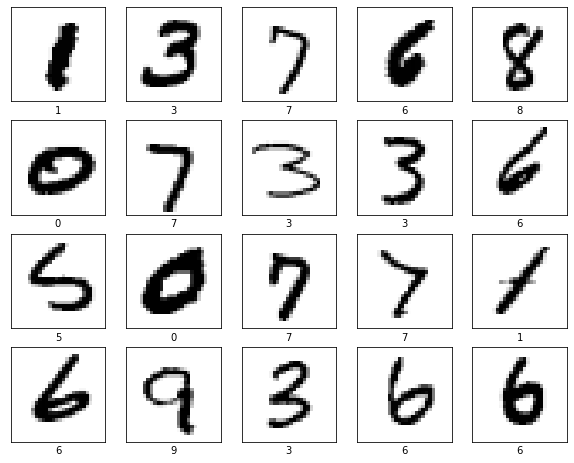
\includegraphics[width=0.75\textwidth]{images/mnist_example.png}}
  \caption{MNIST example}
  \label{fig:mnist_example}
\end{figure}

\subsection{Neural Net Math}
\subsubsection{Forward Propagation}
Since each image is a 28x28 array of values (0-255), each image can be flattened into a 784 length vector. This turns what is previously a $\mathbb{R}^{n\times n}$ matrix into a vector that is in $\mathbb{R}^{n^2}$. Specifically, in the case of MNIST it maps $\mathbb{R}^{28 \times 28} \to \mathbb{R}^{784}$.
\begin{align}
  \begin{bmatrix}
     x_{00 00} & x_{00 01} & \dots & x_{00 26}&  x_{00 27} \\
     x_{01 00} & x_{01 01} & \dots & x_{01 26}&  x_{01 27} \\
     \vdots & \vdots & \vdots & \vdots & \vdots \\
     x_{26 00} & x_{26 01} & \dots & x_{26 26}&  x_{26 27} \\
     x_{27 00} & x_{27 01} & \dots & x_{27 26}&  x_{27 27}
  \end{bmatrix}
  \to
  \begin{bmatrix}
    x_{00 00} & x_{00 01} & \dots x_{27 26}&  x_{27 27} 
 \end{bmatrix}
\end{align}

The neural network will take the input $x$ and it will first pass a linear transformation from the matrix $A^{[0]}$. It then passes through the affine function $Z^{[1]} = w^{[1]} A^{[0]} + b^{[1]}$. In order to extract the next $A$, an activation function transforms $Z$ so $A^{[1]} = g(Z^{[1]})$ where $g(x) = ReLU(x)$ in this case. We then pass it through again and end the activation function with a softmax in order to map to the probabilities.
\begin{align}
  \begin{bmatrix}
     1.3 \\
     5.1 \\
     2.2 \\
     0.7 \\
     1.1
  \end{bmatrix}
  \to 
  \begin{bmatrix}
    \frac{e^{z_i}}{\sum_{j=1}^{K}e^{z_j}}
  \end{bmatrix}
  \to 
  \begin{bmatrix}
    0.02 \\
    0.90 \\
    0.05 \\
    0.01 \\
    0.02
  \end{bmatrix}
\end{align}

\subsubsection{Backward Propagation}
Backward propagation involves using the difference from the calculated solutions to the reality.  Each $A^{[i]}$ is the output from the previous layers of the neural network, and we will assume we have two layers for the MNIST problem to simplify things. In this case, backpropagation will be 

\begin{equation}
  \begin{aligned}
    \partial z^{[2]} = A^{[2]} - Y \\
    \partial W^{[2]} = \frac{1}{m} \partial z^{[2]} A^{[1] \top} \\
    \partial b^{[2]} = \frac{1}{m} \sum \partial z^{2} \\
    \partial z^{[1]} = W^{[2] \top} \partial z^{[2]} \times g^\prime(z^{[1]}) \\
    \partial W^{[1]} = \frac{1}{m} \partial z^{[1]} x^\top \\
    \partial b^{[1]} = \frac{1}{m} \sum \partial z^{[1]}
  \end{aligned}
\end{equation}

\subsubsection{Updates}
These are updated in the gradient descent algorithm with a learning rate $\alpha$ by 
\begin{equation}
  \begin{aligned}
    W^{[1]} := W^{[1]} - \alpha \partial W^{[1]} \\
    b^{[1]} := b^{[1]} - \alpha \partial b^{[1]} \\
    W^{[2]} := W^{[2]} - \alpha \partial W^{[2]} \\
    b^{[2]} := b^{[2]} - \alpha \partial b^{[2]}
  \end{aligned}
\end{equation}